%%%%%%%%%%%%%%%%%%%%%%%%%%%%%%%%%%%%%%%
% Original author:
% Meet Bhatnagar
%
% Original repository:
% https://github.com/MeetDarkPow/meet-Res
%%%%%%%%%%%%%%%%%%%%%%%%%%%%%%%%%%%%%%

\documentclass[]{meetresume-class}


\begin{document}
	
	%%%%%%%%%%%%%%%%%%%%%%%%%%%%%%%%%%%%%%
	%
	%     COLUMN ONE
	%
	%%%%%%%%%%%%%%%%%%%%%%%%%%%%%%%%%%%%%%
	
	\begin{minipage}[t]{0.33\textwidth} 
		\begin{large}
			\headername{Meet Bhatnagar}\\
		\end{large}
		Third Year (B.Tech)\\
		Computer Science $\&$ Engineering\\ 
		at VIT Vellore \\ 
		CGPA : 8.28 till \nth{5} Semester 
		
		
		%%%%%%%%%%%%%%%%%%%%%%%%%%%%%%%%%%%%%%
		%     LINKS
		%%%%%%%%%%%%%%%%%%%%%%%%%%%%%%%%%%%%%%
		\section{Links} 
		\noindent\rule{5cm}{0.6pt}
		
		Github: \href{https://github.com/MeetDarkPow}{\custombold{Profile Link}} \\
		LinkedIn:  \href{https://www.linkedin.com/in/meet-bhatnagar-a41842181/}{\custombold{Profile Link}}
		\sectionsep
		%%%%%%%%%%%%%%%%%%%%%%%%%%%%%%%%%%%%%%
		%     SKILLS
		%%%%%%%%%%%%%%%%%%%%%%%%%%%%%%%%%%%%%%
		\section{Skills}
		\noindent\rule{5cm}{0.6pt}
	
		\subsection{OS}
		Windows
		\vspace{6pt}
		
		\subsection{Languages}
		Proficient: C/C++, R Programming
		%Familiar: HTML, CSS, JavaScript
		\vspace{6pt}
		
		\subsection{Data Science}
		Data Visualization, Data Analysis,\\
		Data Mining, Data Cleaning
		\vspace{6pt}
		
		\subsection{Databases}
		MySQL%, PostgreSQL
		\vspace{6pt}
		
		\subsection{Others}
		R Markdown, GitHub Desktop, RStudio,\\
		MiKTeX, MATLAB%, Sublime Text
		\sectionsep
		%%%%%%%%%%%%%%%%%%%%%%%%%%%%%%%%%%%%%%
		%     COURSEWORK
		%%%%%%%%%%%%%%%%%%%%%%%%%%%%%%%%%%%%%%
		\section{Coursework}
		\noindent\rule{5cm}{0.6pt}
		
		Data Structures\\
		Algorithm\\
		%System Design\\
		%Computer Networks\\
		Operating Systems\\
		DBMS\\
		Data Science
		\sectionsep
		%%%%%%%%%%%%%%%%%%%%%%%%%%%%%%%%%%%%%%
		%     EDUCATION
		%%%%%%%%%%%%%%%%%%%%%%%%%%%%%%%%%%%%%%
		\section{Education} 
		\noindent\rule{5cm}{0.6pt}\\
		\datecolor{2018-Present}
		\subsection{B.Tech. - CSE}
		VIT Vellore, Tamil Nadu \\
		CGPA : 8.28/10\\
		\vspace{8pt}
		\datecolor{2016-2017}
		\subsection{CBSE - Intermediate}
		RKVM, Gwalior (M.P.)\\
		Percentage : 82.2\%\\
		\vspace{8pt}
		\datecolor{2014-2015}
		\subsection{CBSE - High School}
		Dewan Public School, Meerut (U.P.)\\
		CGPA : 10/10
		\sectionsep
		%%%%%%%%%%%%%%%%%%%%%%%%%%%%%%%%%%%%%%
		%     CERTIFICATES
		%%%%%%%%%%%%%%%%%%%%%%%%%%%%%%%%%%%%%%
		\section{Certificates}
		\noindent\rule{5cm}{0.6pt}
		
		Johns Hopkins University - Data Science Specialization (2020/21)\\
		%Duke University - Analytic Techniques for Business Specialization (2021)\\
		%University of Pennsylvania - Positive Psychology Specialization (2021)\\
		
	\end{minipage} 
	\hfill
	%%%%%%%%%%%%%%%%%%%%%%%%%%%%%%%%%%%%%%
	%
	%     COLUMN TWO
	%
	%%%%%%%%%%%%%%%%%%%%%%%%%%%%%%%%%%%%%%
	\begin{minipage}[t]{0.66\textwidth} 
		% \descript{BS in Computer ence}
		\hspace*{0pt}\hfill    \\
		%\hspace*{0pt}\hfill    \\
		%\hspace*{0pt}\hfill J-90, NIT Srinagar, Hazaratbal \\
		%\hspace*{0pt}\hfill Srinagar, J$\&$ K-190 006, India \\
		\hspace*{0pt}\hfill 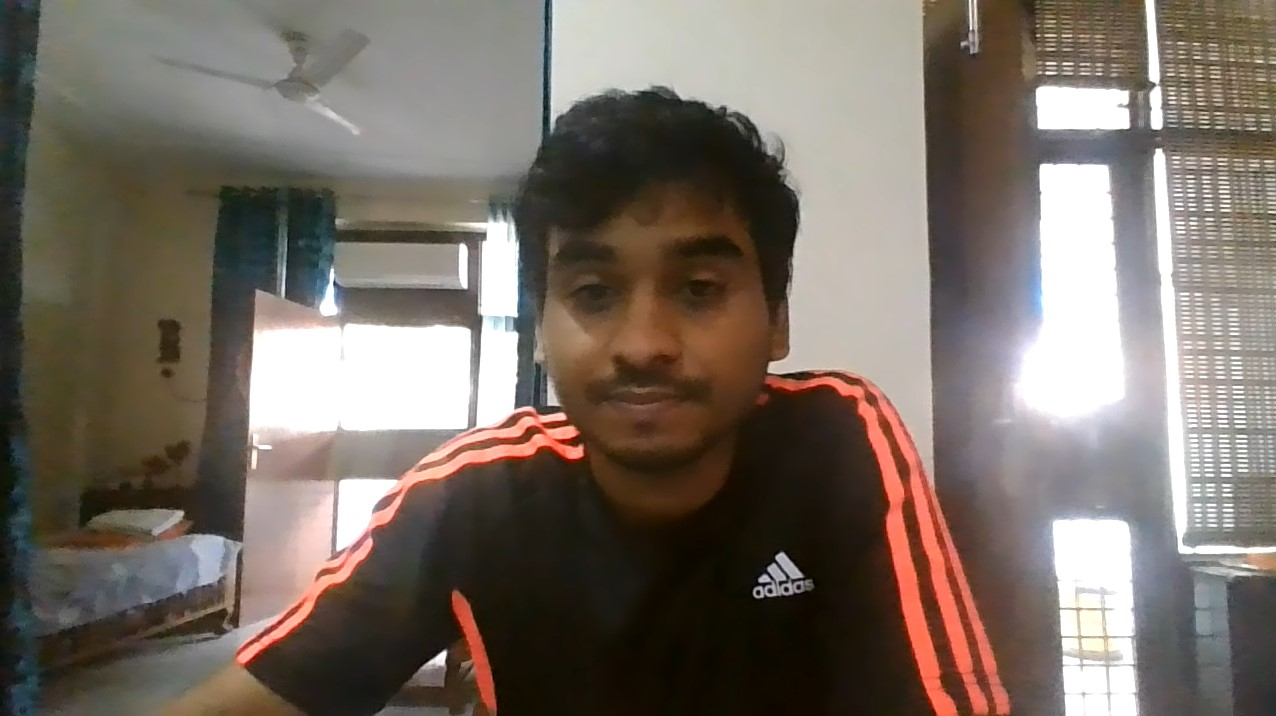
\includegraphics[width=2.5cm, height=2.5cm]{profile-pic.jpg}\\
		\hspace*{0pt}\hfill Mobile : +91-6397356028 \\
		\hspace*{0pt}\hfill Email : \textbf{\href{mailto:meet1708@gmail.com}{meet1708@gmail.com}}
		%\hspace*{0pt}\hfill %Web.:\textbf{\href{http://rahulchauhan.net}{http://rahulchauhan.net}} 
		%%%%%%%%%%%%%%%%%%%%%%%%%%%%%%%%%%%%%%
		%     EXPERIENCE
		%%%%%%%%%%%%%%%%%%%%%%%%%%%%%%%%%%%%%%
		\section{Experience}
		\noindent\rule{12.5cm}{0.4pt}
		\datecolor{20XX-now} \runsubsection{OSGeo}
		\descript{Google Summer of Code 2018 Student Developer Intern }
		\noindent
		\hspace{5em}%
		\begin{minipage}{0.85\textwidth\vspace{2pt}}
			Support of Unit of Measure conversion in istSOS3: My project is to add conversion of
			unit of measure in istsos3. User can convert unit in another specified unit.
		\end{minipage}
		\descriptright{Python, PostgreSQL, Pandas, Numpy, Scipy, Pint, Postgresql-unit, Javascript}
		\sectionsep
		
		\datecolor{20XX-now} \runsubsection{OSGeo}
		\descript{Google Summer of Code 2017 Student Developer Intern }
		\noindent
		\hspace{5em}%
		\begin{minipage}{0.85\textwidth\vspace{2pt}}
			Data analysis and statastical tool suit: istsos2 provides easily manage your sensor network
			and distribute your data in a standard way. which is be used to automate the creation of statisticate
			documents using OAT(Observation analysis tool) and harvesting the data from an istSOS server.
		\end{minipage}
		\descriptright{ExtJS, Dygraph.js, D3.js, Data analysis, Python, PostGIS, Pandas, Numpy, Scipy}
		\sectionsep
		
		\datecolor{20XX-now} \runsubsection{Indian Institute of Science, Banglore}
		\descript{Research Intern}
		\noindent
		\hspace{5em}%
		\begin{minipage}{0.85\textwidth\vspace{2pt}}
			pan sharpening is one kind of data fusion become very wide spread method which populate the spectral band information with the influence of high spatial information.
		\end{minipage}
		\descriptright{Satellite images(Chandrayan), Fusion Algorithm, Java}
		\sectionsep
		
		\datecolor{20XX-now} \runsubsection{Smokey, Banglore}
		\descript{Android Intern}
		\noindent
		\hspace{5em}%
		\begin{minipage}{0.85\textwidth\vspace{2pt}}
			Worked on location based services application which provide services at any location near
			services provider and also made friend module.
		\end{minipage}
		\descriptright{Android, Mysql, Google map}
		%%%%%%%%%%%%%%%%%%%%%%%%%%%%%%%%%%%%%%
		%     AWARDS
		%%%%%%%%%%%%%%%%%%%%%%%%%%%%%%%%%%%%%%
		\section{Achievements/Awards} 
		\noindent\rule{12.5cm}{0.4pt}
		\datecolor{20XX-now} \runsubsection{Rajsthan Hackathon}
		\descript{Participated}
		\noindent
		\hspace{5em}%
		\begin{minipage}{0.85\textwidth\vspace{2pt}}
			In this hackathon Developed distributed Voting Application.
		\end{minipage}
		\datecolor{20XX-now} \runsubsection{Angelhack, Jaipur}
		\descript{Finalist}
		\noindent
		\hspace{5em}%
		\begin{minipage}{0.85\textwidth\vspace{2pt}}
			In this hackathon Developed a Dapp using Blockchain which is based on smart contract.
		\end{minipage}
		\datecolor{20XX-now} \runsubsection{Digital India}
		\descript{Grand Prize Winner}
		\noindent
		\hspace{5em}%
		\begin{minipage}{0.85\textwidth\vspace{2pt}}
			In this hackathon developed a web-app in which showing kashmir as paradise on earth.
		\end{minipage}
		%%%%%%%%%%%%%%%%%%%%%%%%%%%%%%%%%%%%%%
		%     SIDE PROJECT
		%%%%%%%%%%%%%%%%%%%%%%%%%%%%%%%%%%%%%%
		\section{Side Project}
		\noindent\rule{12.5cm}{0.4pt}
		\datecolor{20XX-now} \runsubsection{Digital Certificate Dapp using Ethereum}
		\descript{Blockchain, Web3JS}
		\noindent
		\hspace{5em}%
		\begin{minipage}{0.85\textwidth\vspace{5pt}}
			A Dapp issue certificate and verify. An Idea to use Blockchain to create Digital Certificate.
		\end{minipage}
		\datecolor{20XX-now} \runsubsection{Identifying Gender From Images of Faces}
		\descript{ML}
		\noindent
		\hspace{5em}%
		\begin{minipage}{0.85\textwidth\vspace{5pt}}
			Identifying gender of a person by looking at his/her Photograph.
		\end{minipage}
		\datecolor{20XX-now} \runsubsection{Small Project}
		\descript{Android, Data Analysis, Image Processing}
		\noindent
		\hspace{5em}%
		\begin{minipage}{0.85\textwidth\vspace{5pt}}
			Result Portal, Voice Calci, Cubic Bispline, Image Compression, smoothing, Fitting Curve.
		\end{minipage}
	\end{minipage} 
\end{document}  \documentclass[]{article}